% =====================================================================
% Manuscrito para submissão à REVISTA BRASILEIRA DE NEUROLOGIA (RBN)
% Tipo: Artigo Original
% Versão independente, autossuficiente — SEM vínculo com working papers,
% repositórios ou marcas externas. Formatado segundo as
% "Instruções para os autores" da RBN (v. 60, n. 3, 2024):
%   - até 4.000 palavras (excluindo resumo, figuras e tabelas)
%   - máximo de 3 figuras e 4 tabelas/quadros
%   - até 75 referências, estilo Vancouver, numeradas por ordem de citação
%   - estrutura: Introdução, Material e Métodos, Resultados, Discussão,
%     Conclusão, Agradecimentos
%   - resumo estruturado de até 250 palavras + até 7 descritores (DeCS)
%   - Times New Roman/Arial 12, espaçamento 1,5, páginas numeradas
%
% >>> A PREENCHER PELOS AUTORES ANTES DA SUBMISSÃO (não inventados aqui):
%   - ORCID de cada autor
%   - afiliação institucional completa (até três níveis), cidade, estado, país
%   - titulação e cargo atual de cada autor
%   - e-mail do autor correspondente
% Esses campos aparecem no texto marcados como [A PREENCHER].
%
% Compilação: pdflatex equipamentos-rm-parkinson-RBN.tex (2x)
% =====================================================================

\documentclass[12pt,a4paper,oneside]{article}

\usepackage[T1]{fontenc}
\usepackage[utf8]{inputenc}
\usepackage[brazilian]{babel}
\usepackage{newtxtext}     % Times New Roman (exigência RBN)
\usepackage{newtxmath}
\usepackage[section]{placeins}
\usepackage[a4paper,top=2.5cm,bottom=2.5cm,left=3cm,right=2.5cm]{geometry}
\usepackage{setspace}
\usepackage{indentfirst}
\usepackage{titlesec}
\usepackage{caption}
\usepackage{booktabs}
\usepackage{array}
\usepackage{graphicx}
\usepackage{xcolor}
\usepackage{lastpage}
\usepackage{fancyhdr}
\usepackage[colorlinks=true,urlcolor=blue!55!black,linkcolor=black,
            citecolor=black,breaklinks=true]{hyperref}
\usepackage{url}
\usepackage{xurl}
\Urlmuskip=0mu plus 1mu\relax

\graphicspath{{figures-equipamentos-rm/}}

\onehalfspacing                       % espaçamento 1,5 (exigência RBN)
\setlength{\parindent}{1.25cm}
\setlength{\parskip}{0pt}

\titleformat{\section}{\normalfont\bfseries\large\uppercase}{\thesection}{0.6em}{}
\titleformat{\subsection}{\normalfont\bfseries\normalsize}{\thesubsection}{0.6em}{}
\titlespacing*{\section}{0pt}{16pt}{8pt}
\titlespacing*{\subsection}{0pt}{10pt}{5pt}

\captionsetup[table]{labelfont=bf,name=Tabela,labelsep=endash,
                     position=above,justification=centering,font=small}
\captionsetup[figure]{labelfont=bf,name=Figura,labelsep=endash,
                      position=below,justification=centering,font=small}
\captionsetup{skip=6pt}

% paginação obrigatória (todas as páginas numeradas)
\pagestyle{fancy}\fancyhf{}
\fancyfoot[C]{\small\thepage}
\renewcommand{\headrulewidth}{0pt}

% mecanismo de referências numéricas estilo Vancouver (por ordem de citação)
\newcounter{bibctr}
\newcommand{\refitem}[1]{\refstepcounter{bibctr}\noindent%
  \hangindent=0.7cm\hangafter=1\label{#1}\textbf{\thebibctr.}\ }

\begin{document}

% =====================================================================
% PÁGINA DE ROSTO
% =====================================================================
\thispagestyle{fancy}
\begin{singlespace}

\begin{center}
{\small\textsc{Artigo Original \quad\textbar\quad Revista Brasileira de Neurologia}}

\vspace{12pt}
{\large\bfseries Iniquidade regional no acesso à neuroimagem para a
doença de Parkinson no Brasil: análise do parque instalado no CNES
(2013\textendash 2025)\par}

\vspace{8pt}
{\itshape Regional inequity in access to neuroimaging for Parkinson's
disease in Brazil: an analysis of the installed capacity in the CNES
(2013\textendash 2025)\par}

\vspace{8pt}
{\footnotesize\textbf{Título abreviado:} Neuroimagem e Parkinson no
SUS \quad\textbar\quad \textbf{Short title:} Neuroimaging for PD in
Brazil}

\vspace{14pt}
\textbf{Leonardo Chalhoub} \quad\textbullet\quad \textbf{Alexandre Maciel Rolim}\\[4pt]
\textbf{Luis Fernando Kranz} \quad\textbullet\quad \textbf{Jefferson Korte}
\end{center}

\vspace{0.4cm}
\small
\noindent Todos os autores atuam como \textbf{pesquisadores
independentes}, Brasil.\\[4pt]
\noindent\textbf{Titulação, cargo atual e ORCID:}\\[2pt]
\noindent\textit{Leonardo Chalhoub} \textemdash{} Pesquisador
independente; \textit{Expert Data Engineer}. Mestre em Administração
(Finanças), Universidade Federal do Rio Grande do Sul (UFRGS);
graduando em Engenharia de Software, Universidade Estácio de Sá
(2023\textendash 2026). Rio de Janeiro, RJ, Brasil.
ORCID: 0000-0003-0484-158X.\\[2pt]
\noindent\textit{Alexandre Maciel Rolim} \textemdash{} Pesquisador
independente; Tecnólogo em Radiologia. Mestre em Proteção Radiológica,
Instituto Federal de Santa Catarina (IFSC). Florianópolis, SC, Brasil.
ORCID: 0009-0000-3983-4713.\\[2pt]
\noindent\textit{Luis Fernando Kranz} \textemdash{} Pesquisador
independente; Tecnólogo em Radiologia. Mestre em Administração,
Universidade Federal do Rio Grande do Sul (UFRGS). Porto Alegre, RS,
Brasil. ORCID: 0009-0009-6015-3141.\\[2pt]
\noindent\textit{Jefferson Korte} \textemdash{} Pesquisador
independente; estudante de Ciência da Computação, Universidade
Tecnológica Federal do Paraná (UTFPR). Curitiba, PR, Brasil.
ORCID: 0009-0006-9466-9830.

\vspace{0.5cm}
\noindent\textbf{Autor correspondente:} Leonardo Chalhoub
(pesquisador independente; \textit{Expert Data Engineer}).
E-mail: leochalhoub@hotmail.com.

\vspace{0.5cm}
\noindent\textbf{Declaração de conflito de interesses:} os autores
declaram não haver conflito de interesses.

\vspace{0.2cm}
\noindent\textbf{Declaração de financiamento:} o presente estudo não
recebeu financiamento de qualquer fonte pública, privada ou sem fins
lucrativos.

\vspace{0.2cm}
\noindent\textbf{Contribuições dos autores (taxonomia CRediT):}
\textit{L.\ Chalhoub} \textemdash{} Conceituação; Curadoria de dados;
Análise formal; \textit{Software}; Metodologia (componente de dados);
Visualização; Redação (rascunho original das seções analíticas);
Redação (revisão e edição). \textit{A.\,M.\ Rolim} \textemdash{}
Metodologia (componente clínico-epidemiológico); Investigação
(revisão da literatura clínica); Validação; Redação (rascunho original
das seções clínicas); Redação (revisão e edição). \textit{L.\,F.\
Kranz} \textemdash{} Conceituação; Metodologia; Validação; Supervisão;
Redação (revisão e edição). \textit{J.\ Korte} \textemdash{}
\textit{Software}; Curadoria de dados; Visualização; Redação (revisão
e edição). Todos os autores aprovaram a versão final e respondem pela
integridade do trabalho. \textit{(Distribuição de papéis a confirmar
pelos autores.)}

\vspace{0.2cm}
\noindent\textbf{Aspectos éticos:} estudo ecológico baseado
exclusivamente em dados administrativos públicos, agregados e
anonimizados (CNES/DATASUS e IBGE), sem identificação de indivíduos.
Conforme a Resolução CNS n.\ 510/2016, pesquisas que utilizam
informações de acesso público e sem identificação de participantes
são dispensadas de apreciação pelo Sistema CEP/CONEP, não havendo,
portanto, número CAAE aplicável.

\vspace{0.2cm}
\noindent\textbf{Disponibilidade de dados e reprodutibilidade:} todos
os dados primários utilizados são de acesso público e gratuito,
disponibilizados pelo DATASUS (microdados do CNES) e pelo IBGE
(estimativas e projeções populacionais). O código-fonte completo do
\textit{pipeline} de processamento e o conjunto de dados consolidado
(camada \textit{gold}, versionado e acompanhado de suíte de testes
automatizados) estão publicamente disponíveis no repositório aberto do
projeto,\footnote{Repositório do projeto:
\url{https://github.com/leonardochalhoub/mirante-dos-dados-br}.}
permitindo reprodução integral por terceiros sem custo marginal.

\vspace{0.2cm}
\noindent\textbf{Uso de inteligência artificial:} ferramentas de
inteligência artificial foram empregadas exclusivamente como apoio à
edição de linguagem e à formatação do manuscrito. Não foram
utilizadas na coleta, no processamento ou na análise dos dados. Os
autores revisaram integralmente o conteúdo e respondem pela ausência
de erros, plágio ou viés.

\end{singlespace}

\newpage

% =====================================================================
% RESUMO (estruturado) + DESCRITORES
% =====================================================================
\section*{Resumo}
\begin{singlespace}\small\noindent
\textbf{Introdução.} A doença de Parkinson (DP) é a condição
neurodegenerativa de crescimento mais acelerado no mundo; no Brasil,
estima-se 535.999 casos em 2024, com projeção de 1.250.638 em 2060.
O diagnóstico diferencial entre DP idiopática e parkinsonismos
atípicos requer suporte de neuroimagem escalonada (ressonância
magnética, tomografia computadorizada, DAT-SPECT e PET/CT).
\textbf{Objetivo.} Quantificar e caracterizar a distribuição
regional do parque instalado dessas quatro modalidades no Brasil e
avaliar a equidade do acesso. \textbf{Material e métodos.} Estudo
ecológico de série temporal (2013\textendash 2025) a partir dos
microdados mensais do Cadastro Nacional de Estabelecimentos de Saúde
(CNES/DATASUS), com normalização por milhão de habitantes (Mhab) com
base em estimativas do IBGE, \textit{benchmarking} internacional
(OCDE), índice de Kakwani sobre densidade de ressonância magnética
(RM) \textit{versus} Índice de Desenvolvimento Humano (IDH) estadual
e índice de necessidade (casos estimados de DP por equipamento).
\textbf{Resultados.} A densidade nacional de RM atingiu 18,3/Mhab em
2025, alinhada à mediana da OCDE (19,4), porém com forte gradiente
interno: 17 das 27 unidades federativas (UF) situam-se abaixo da
mediana da OCDE, e Acre (5,7), Roraima (8,1) e Amazonas (8,6) abaixo
de metade desse referencial. O índice de Kakwani foi $+0{,}183$
(IC 95\,\% [$+0{,}12;+0{,}24$]), indicando distribuição regressiva
pró-rico. O índice de necessidade variou cerca de nove vezes entre
extremos. \textbf{Conclusão.} A barreira ao diagnóstico diferencial
da DP no Brasil não é o volume agregado, mas a iniquidade espacial do
acesso, que tende a se agravar com o envelhecimento populacional.

\vspace{0.35cm}\noindent\textbf{Descritores:} Doença de Parkinson;
Neuroimagem; Imageamento por Ressonância Magnética; Tomografia
Computadorizada de Emissão de Fóton Único; Sistema Único de Saúde;
Disparidades em Assistência à Saúde; Sistemas de Informação em Saúde.
\end{singlespace}

\section*{Abstract}
\begin{singlespace}\small\noindent
\textbf{Introduction.} Parkinson's disease (PD) is the fastest-growing
neurodegenerative condition worldwide; Brazil is estimated to have had
535,999 cases in 2024, projected to reach 1,250,638 by 2060. The
differential diagnosis between idiopathic PD and atypical parkinsonisms
requires tiered neuroimaging support (magnetic resonance imaging,
computed tomography, DAT-SPECT and PET/CT). \textbf{Objective.} To
quantify and characterize the regional distribution of the installed
capacity of these four modalities in Brazil and to assess equity of
access. \textbf{Material and methods.} Ecological time-series study
(2013\textendash 2025) based on monthly microdata from the National
Registry of Health Establishments (CNES/DATASUS), normalized per
million population (Mpop) using IBGE estimates, with international
benchmarking (OECD), a Kakwani index on MRI density \textit{versus}
state Human Development Index (HDI), and a need index (estimated PD
cases per device). \textbf{Results.} National MRI density reached
18.3/Mpop in 2025, aligned with the OECD median (19.4), but with a
steep internal gradient: 17 of 27 federal units (FU) fall below the
OECD median, and Acre (5.7), Roraima (8.1) and Amazonas (8.6) below
half of that benchmark. The Kakwani index was $+0.183$
(95\,\% CI [$+0.12;+0.24$]), indicating a pro-rich regressive
distribution. The need index varied roughly nine-fold between
extremes. \textbf{Conclusion.} The barrier to PD differential
diagnosis in Brazil is not aggregate volume but the spatial inequity
of access, which is likely to worsen with population ageing.

\vspace{0.35cm}\noindent\textbf{Keywords:} Parkinson Disease;
Neuroimaging; Magnetic Resonance Imaging; Tomography, Emission-Computed,
Single-Photon; Unified Health System; Healthcare Disparities; Health
Information Systems.
\end{singlespace}

\newpage

% =====================================================================
\section{Introdução}
% =====================================================================

A doença de Parkinson (DP) é a condição neurodegenerativa de
crescimento populacional mais acelerado no mundo. O estudo
\textit{Global Burden of Disease} estima que o número de pessoas com
DP saltou de 3,15 milhões em 1990 para 11,77 milhões em 2021, e
projeções recentes apontam para cerca de 25 milhões em 2050,
configurando o que diversos autores descrevem como uma
``pandemia de Parkinson''\,[\ref{ref:gbd}, \ref{ref:su}]. A pressão
não se restringe aos países de alta renda: os Estados Unidos projetam
a duplicação do número de casos \textemdash{} de cerca de 680 mil em
2010 para 1,2 milhão em 2030\,[\ref{ref:marras}] \textemdash{} e a
Europa registra prevalência de 160 a 250 por 100 mil
habitantes\,[\ref{ref:voncamp}], mas o maior crescimento relativo
concentra-se em países de renda média, simultaneamente pressionados
pelo envelhecimento populacional e por sistemas de saúde em
consolidação \textemdash{} contexto em que o Brasil se insere.

Para o Brasil, a evidência epidemiológica era fragmentada até
recentemente. O estudo longitudinal ELSI-Brazil (\textit{Estudo
Longitudinal da Saúde dos Idosos Brasileiros}), publicado em 2025,
estimou prevalência de 0,84\,\% (IC 95\,\%: 0,64\textendash 1,09)
entre indivíduos com 50 anos ou mais, com aumento exponencial com a
idade (de 0,39\,\% aos 50\textendash 59 anos para 2,75\,\% acima de 80
anos) e maior acometimento masculino (razão de chances 2,35). Com base
nessa prevalência e nas projeções populacionais do IBGE, os autores
estimaram 535.999 casos em 2024 (IC 95\,\%: 309.963\textendash 922.948),
projetando 1.250.638 casos até 2060 \textemdash{} acréscimo médio de
19.851 casos por ano\,[\ref{ref:elsi}]. Esses números configuram
desafio crescente para o Sistema Único de Saúde (SUS) e o setor
suplementar, em paralelo ao envelhecimento populacional projetado
pelo IBGE para as próximas duas décadas\,[\ref{ref:ibge-proj}].

O diagnóstico de DP é fundamentalmente clínico, ancorado nos
critérios da \textit{Movement Disorder Society} (MDS) de
2015\,[\ref{ref:mds}]. O desafio reside no diagnóstico
\textbf{diferencial} entre a DP idiopática e os parkinsonismos
atípicos \textemdash{} atrofia multissistêmica (AMS), paralisia
supranuclear progressiva (PSP), demência com corpos de Lewy (DCL) e
degeneração corticobasal (DCB) \textemdash{}, cujas apresentações
iniciais se sobrepõem à da DP e cuja distinção precoce tem
implicações prognósticas e terapêuticas relevantes\,[\ref{ref:tolosa}].
Nesses cenários de incerteza, todas as principais diretrizes
internacionais recomendam o suporte da neuroimagem\,[\ref{ref:efns},
\ref{ref:aan}].

O \textit{stack} diagnóstico é hierárquico e escalonado
(Tabela~\ref{tab:stack}). A \textbf{ressonância magnética (RM)} é o
suporte de primeira linha: sequências convencionais (T1, T2, FLAIR)
excluem mimetizadores estruturais, enquanto a imagem ponderada por
susceptibilidade (SWI) revela o sinal da ``cauda de andorinha''
(\textit{swallow-tail sign}) \textemdash{} a perda da hiperintensidade
do nigrossomo-1 na \textit{substantia nigra} \textemdash{}, com
sensibilidade de 94,6\,\% e especificidade de 94,4\,\% para
discriminar DP de controles\,[\ref{ref:swallow}]; sequências
sensíveis à neuromelanina quantificam a depleção dopaminérgica
nigral\,[\ref{ref:pyatigorskaya}]. A \textbf{tomografia computadorizada
(CT)} cumpre papel de exclusão de mimetizadores quando a RM é
indisponível ou contraindicada, além de detectar calcificações dos
gânglios da base\,[\ref{ref:saba}]. A \textbf{DAT-SPECT}, adquirida
em câmara gama com \textsuperscript{123}I-Ioflupano (ou
\textsuperscript{99m}Tc-TRODAT, no mercado brasileiro), quantifica o
transportador dopaminérgico presináptico e é a modalidade mais
específica para distinguir a DP de mimetizadores não degenerativos
(tremor essencial, parkinsonismo medicamentoso): a concordância com o
diagnóstico clínico atinge cerca de 90\,\% nos casos inicialmente
incertos\,[\ref{ref:catafau}, \ref{ref:djang}], e a demonstração de
neuroimagem dopaminérgica \textit{normal} constitui critério de
\textbf{exclusão absoluta} de DP nos critérios MDS\,[\ref{ref:mds},
\ref{ref:ioflupane}]. A \textbf{PET/CT}, modalidade mais avançada e
cara, fornece imagem metabólica (\textsuperscript{18}F-FDG) e
dopaminérgica (\textsuperscript{18}F-DOPA, \textsuperscript{11}C-
raclopride) e cumpre papel terciário, restrito a centros de
referência\,[\ref{ref:stoessl}].

\begin{table}[htbp]
\centering
\caption{Modalidades de neuroimagem no diagnóstico diferencial da
doença de Parkinson, principais achados e códigos correspondentes no
CNES}
\small
\begin{tabular}{@{}p{2.0cm}p{6.2cm}p{2.5cm}p{1.0cm}@{}}
\toprule
\textbf{Modalidade} & \textbf{Papel no diagnóstico diferencial e
achado-chave} & \textbf{Acurácia / nível} & \textbf{CNES} \\
\midrule
Ressonância magnética & Exclusão de mimetizadores estruturais; SWI
para o sinal da ``cauda de andorinha'' (perda do nigrossomo-1);
neuromelanina quantifica a depleção nigral & Sens.\ 94,6\,\%, espec.\
94,4\,\% (SWI); 1ª linha & 1:12 \\
Tomografia computadorizada & Exclusão de mimetizadores quando a RM é
indisponível/contraindicada; calcificações dos gânglios da base &
Alternativa & 1:11 \\
DAT-SPECT (câmara gama) & Quantifica o transportador dopaminérgico
presináptico; exame \textit{normal} $=$ exclusão absoluta de DP
(MDS 2015) & Concordância $\sim$90\,\% em casos incertos; 2ª linha &
1:01 \\
PET/CT & Imagem metabólica (\textsuperscript{18}F-FDG) e dopaminérgica
(\textsuperscript{18}F-DOPA, \textsuperscript{11}C-raclopride);
centros de referência & 3ª linha & 1:18 \\
\bottomrule
\end{tabular}
\par\noindent{\small Fonte: elaboração própria; códigos conforme o
catálogo de equipamentos do CNES/DATASUS. Chave CNES:
\texttt{(TIPEQUIP:CODEQUIP)}.}
\label{tab:stack}
\end{table}

A literatura nacional tem explorado a infraestrutura diagnóstica sob
lentes parciais \textemdash{} análises espaciais isoladas do acesso a
equipamentos de imagem\,[\ref{ref:lopes}] ou abordagens estritamente
clínicas em diretrizes\,[\ref{ref:saba}]. Falta uma análise que
articule, de forma reproduzível, a oferta instalada das modalidades
de neuroimagem relevantes para a DP com a sua distribuição regional e
a equidade do acesso. O presente estudo tem por objetivo: (i)
quantificar o parque nacional de RM, CT, PET/CT e câmaras gama
cadastrado no Cadastro Nacional de Estabelecimentos de Saúde (CNES),
por unidade federativa (UF), ano e setor; (ii) comparar a densidade
brasileira com referenciais internacionais; e (iii) caracterizar a
iniquidade regional do acesso por meio de mapas e índices formais de
equidade.

% =====================================================================
\section{Material e métodos}
% =====================================================================

\subsection{Desenho e fontes de dados}

Trata-se de estudo ecológico, descritivo-analítico, de série temporal,
fundamentado em microdados administrativos públicos de cobertura
nacional. A fonte primária é o módulo de Equipamentos do CNES,
mantido pelo DATASUS/Ministério da Saúde, que disponibiliza microdados
mensais por estabelecimento de saúde (arquivos
\texttt{EQ<UF><ano><mês>} no formato DBC). Cada equipamento é
identificado pelas chaves \texttt{TIPEQUIP} (categoria) e
\texttt{CODEQUIP} (código dentro da categoria), conforme o catálogo
oficial do DATASUS\,[\ref{ref:datasus-cat}]. A janela de análise é
2013\textendash 2025, escolhida por consistência da série após a
padronização das tabelas de procedimentos do SUS. As estimativas
anuais de população residente por UF, utilizadas na normalização per
capita, provêm do IBGE (SIDRA, Tabela 6579)\,[\ref{ref:ibge-pop}].

As quatro modalidades de interesse foram delimitadas pelas chaves
\texttt{(TIPEQUIP, CODEQUIP)}: \texttt{1:12} para RM, \texttt{1:11}
para CT, \texttt{1:18} para PET/CT e \texttt{1:01} para câmara gama
(suporte da DAT-SPECT). Como a câmara gama abrange aplicações além da
DAT-SPECT (cintilografia óssea, miocárdica e tireoidiana), o parque
total dessa categoria é interpretado como limite superior da
capacidade potencialmente alocável à DAT-SPECT.

\subsection{Processamento e indicadores}

Os microdados foram processados por um \textit{pipeline} aberto e
reproduzível, organizado segundo a arquitetura \textit{medallion}
(camadas \textit{bronze}, \textit{silver} e
\textit{gold})\,[\ref{ref:lakehouse}], implementada em Apache
Spark\,[\ref{ref:spark}] sobre o formato de tabela transacional aberto
Delta Lake\,[\ref{ref:delta}], na plataforma Databricks Free Edition.
Na camada \textit{bronze}, cada arquivo DBC foi convertido para formato
colunar (via \textit{PySUS}/\texttt{pyreaddbc}), preservando os
registros da fonte sem inferência de tipo. Na camada \textit{silver},
os dados foram agregados pela chave composta
\texttt{(UF, ano, TIPEQUIP, CODEQUIP)}, com normalização de tipos,
deduplicação por estabelecimento (\texttt{COUNT(DISTINCT CNES)}) e
separação das contagens entre SUS e setor privado pela variável
\texttt{IND\_SUS}. Na camada \textit{gold}, acrescentou-se a população
do IBGE para o cálculo da densidade por milhão de habitantes (/Mhab).
O código-fonte do \textit{pipeline}, o conjunto consolidado versionado
e a suíte de testes automatizados que asseguram a reprodutibilidade
estão publicamente disponíveis no repositório aberto do projeto (ver
declaração de disponibilidade de dados).

Para cada combinação \texttt{(UF, ano, modalidade)} computaram-se:
a contagem média anual de unidades cadastradas; o número de
estabelecimentos distintos; a partição SUS/privado; e a densidade por
milhão de habitantes. A densidade nacional foi comparada às medianas
da OCDE (\textit{Health at a Glance}) e a referenciais de Estados
Unidos, Japão e Canadá\,[\ref{ref:oecd}, \ref{ref:oecd-ct},
\ref{ref:cadth}, \ref{ref:japan}].

\subsection{Análise de equidade}

A iniquidade regional foi caracterizada por três instrumentos. O
\textbf{coeficiente de variação} inter-UF da densidade per capita foi
calculado por ano como medida de desigualdade relativa. O
\textbf{índice de Kakwani}\,[\ref{ref:kakwani}], instrumento clássico
da Economia da Saúde\,[\ref{ref:wagstaff}], mede a divergência entre a
distribuição cumulativa da densidade de RM e a do Índice de
Desenvolvimento Humano (IDH) estadual 2024\,[\ref{ref:atlas}], usado
como \textit{proxy} de capacidade econômica: $K = C_{\text{RM}} -
G_{\text{IDH}}$, em que $C_{\text{RM}}$ é o índice de concentração de
RM ordenado por IDH crescente e $G_{\text{IDH}}$ é o índice de Gini do
IDH. Valores positivos indicam distribuição regressiva pró-rico
(RM concentrada nas UF de maior IDH); valores negativos indicam
distribuição progressiva pró-pobre. Os intervalos de confiança de
95\,\% foram obtidos por \textit{bootstrap} (1.000 reamostragens).
Por fim, um \textbf{índice de necessidade} confrontou a carga
estimada de DP por UF (população residente $\times$ 0,33\,\%, proxy
simplificada derivada do ELSI-Brazil) com o parque de RM disponível,
expresso como número médio de pacientes com DP por equipamento.

\subsection{Limitações}

A contagem do CNES reflete equipamentos \textit{cadastrados}, não
necessariamente \textit{em operação}; adotou-se a variável de
existência cadastral por alinhamento às convenções internacionais
(OCDE). O cadastro pode duplicar equipamentos quando um mesmo aparelho
é registrado por estabelecimentos parceiros; o \textit{pipeline}
mitiga esse efeito por contagem de estabelecimentos distintos, mas
resíduos podem persistir em UF com forte concentração de pequenos
estabelecimentos. As subcategorias por intensidade de campo magnético
(0,5/1,5/3\,T) e por número de canais de CT foram introduzidas
recentemente no esquema oficial e ainda não são preenchidas em volume
material, o que impede a estratificação por intensidade de campo a
partir apenas do CNES. A proxy de carga de DP (0,33\,\% da população
total) é uma simplificação; refinamentos futuros devem ponderar a
pirâmide etária por UF.

% =====================================================================
\section{Resultados}
% =====================================================================

\subsection{Visão agregada do parque instalado}

Em 2025, o parque nacional das quatro modalidades soma 28.155 unidades
(Tabela~\ref{tab:agregado}), distribuídas em três ordens de grandeza:
câmaras gama (16.089), CT (8.000), RM (3.900) e PET/CT (166). A
composição SUS \textit{versus} privado varia acentuadamente por
modalidade: a câmara gama é 94\,\% SUS \textemdash{} reflexo da
concentração histórica da medicina nuclear na rede pública e
universitária \textemdash{}, enquanto RM (48\,\% SUS) e CT (51\,\%
SUS) aproximam-se do equilíbrio entre os setores, refletindo a
existência de um mercado ambulatorial privado robusto para essas
modalidades.

\begin{table}[htbp]
\centering
\caption{Parque nacional de neuroimagem relevante para a doença de
Parkinson \textendash{} Brasil, 2025}
\begin{tabular}{lrrrr}
\toprule
\textbf{Modalidade} & \textbf{Unidades} & \textbf{SUS} & \textbf{Privado} & \textbf{/Mhab} \\
\midrule
Câmara gama (DAT-SPECT)      & 16.089 & 15.124 & 965   & 75,4 \\
Tomografia computadorizada   &  8.000 &  4.080 & 3.920 & 37,5 \\
Ressonância magnética        &  3.900 &  1.860 & 2.040 & 18,3 \\
PET/CT                       &    166 &     91 &    75 &  0,8 \\
\midrule
\textbf{Total}               & \textbf{28.155} & \textbf{21.155} & \textbf{7.000} & \textbf{132,0} \\
\bottomrule
\end{tabular}
\par\noindent{\small Fonte: elaboração própria a partir dos microdados
do CNES/DATASUS (referência de dezembro de 2025). Densidade por milhão
de habitantes (/Mhab) com base na população residente estimada pelo
IBGE para 2024 (213,4 milhões).}
\label{tab:agregado}
\end{table}

Entre 2013 e 2025, a RM cresceu de 1.654 para 3.900 unidades
($+135\,\%$) e a CT de 3.581 para 8.000 ($+123\,\%$); a PET/CT partiu
de um parque incipiente para 166 unidades, permanecendo escassa: nove
UF têm zero ou uma única unidade em 2025.

O gradiente de participação SUS entre as modalidades tem leitura
clínica direta. A quase totalidade pública da câmara gama (94\,\% SUS)
decorre da centralização histórica da medicina nuclear \textemdash{}
dispendiosa e dependente de radiofármacos \textemdash{} em hospitais
universitários e centros públicos; já a maior penetração privada em RM
e CT reflete o vigor do mercado ambulatorial dessas modalidades. Como
a DAT-SPECT, exame-chave para a exclusão absoluta de DP, depende da
câmara gama, sua oferta efetiva está concentrada na rede pública de
maior complexidade, o que tende a deixar pacientes de UF sem centros
de medicina nuclear sem acesso a esse recurso diagnóstico. A escassez
da PET/CT é ainda mais aguda: com densidade nacional de apenas
0,8/Mhab e nove UF com nenhuma ou uma única unidade, o nível
terciário do \textit{stack} permanece, na prática, indisponível para
parcela expressiva do território.

\subsection{Densidade per capita e comparação internacional}

A densidade nacional de RM atingiu 18,3/Mhab em 2025, cruzando a
mediana da OCDE (19,4/Mhab) por volta de 2024 (Figura~\ref{fig:oecd}).
A Tabela~\ref{tab:internacional} contextualiza esse resultado: em RM,
o Brasil situa-se em posição praticamente mediana entre os 38 países
da OCDE, acima de França (17,6), Reino Unido (14,9) e Canadá (10,8),
porém muito abaixo de Estados Unidos ($\sim$38) e Japão ($\sim$57,
líder da OCDE). Em CT, a densidade brasileira (37,5/Mhab) supera a
mediana da OCDE (27,8), aproximando-se de Estados Unidos e Alemanha
\textemdash{} reflexo do investimento histórico nessa modalidade, mais
antiga e barata, durante a expansão hospitalar das décadas de 1990 e
2000.

\begin{figure}[htbp]
\centering
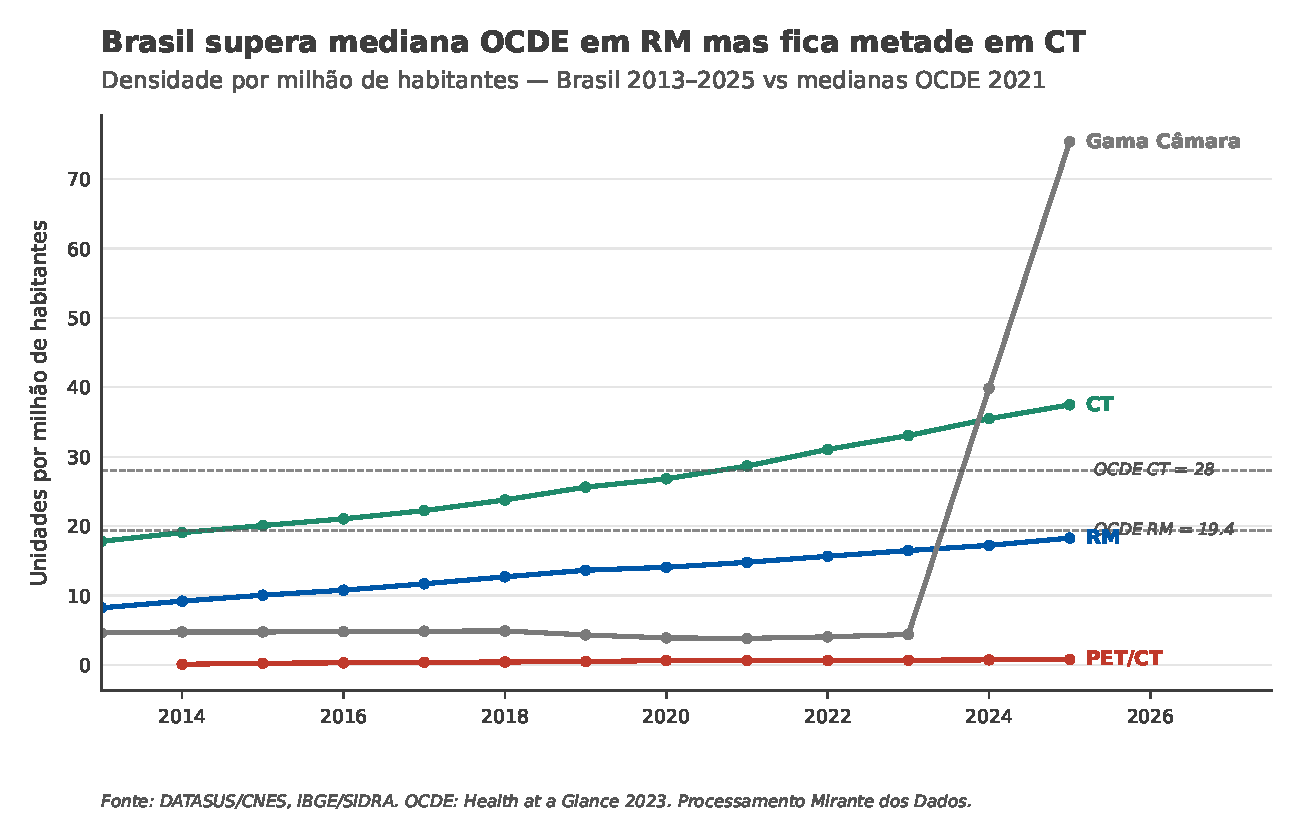
\includegraphics[width=0.9\linewidth]{fig04-density-oecd}
\caption{Densidade per capita das quatro modalidades no Brasil
(2013\textendash 2025) comparada às medianas da OCDE}
\label{fig:oecd}
\par\noindent{\small Fonte: elaboração própria a partir do CNES/DATASUS
e do IBGE; medianas da OCDE conforme \textit{Health at a Glance}
\,[\ref{ref:oecd}].}
\end{figure}

\begin{table}[htbp]
\centering
\caption{Densidade de equipamentos de imagem por milhão de habitantes
\textendash{} comparação internacional (OCDE, 2021\textendash 2023)}
\begin{tabular}{lrr}
\toprule
\textbf{País / agregado} & \textbf{RM /Mhab} & \textbf{CT /Mhab} \\
\midrule
Japão                          & $\sim$57 & 115  \\
Estados Unidos                 & $\sim$38 & 44   \\
Alemanha                       & 35,2     & 35,7 \\
Itália                         & 31,2     & 34,2 \\
Coreia do Sul                  & 29,9     & 41,2 \\
\textbf{Mediana OCDE (38)}     & \textbf{19,4} & \textbf{27,8} \\
França                         & 17,6     & 19,5 \\
Reino Unido                    & 14,9     & 13,5 \\
Canadá                         & 10,8     & 14,1 \\
\midrule
\textbf{Brasil (2025)}         & \textbf{18,3} & \textbf{37,5} \\
\bottomrule
\end{tabular}
\par\noindent{\small Fontes: OCDE \textit{Health at a Glance} 2023;
OCDE \textit{Health Statistics} (CT); \textit{Canadian Medical Imaging
Inventory} 2022\textendash 2023\,[\ref{ref:oecd}, \ref{ref:oecd-ct},
\ref{ref:cadth}]. Brasil computado a partir do CNES/DATASUS.}
\label{tab:internacional}
\end{table}

\subsection{Distribuição regional e gradiente Norte\textendash Sudeste}

A média nacional, contudo, oculta forte heterogeneidade interna. O
mapa coroplético da densidade de RM por UF (Figura~\ref{fig:choro})
evidencia um gradiente Norte\textendash Sudeste: o Distrito Federal e
os estados do Sudeste, Sul e Centro-Oeste concentram as maiores
densidades, ao passo que o eixo Norte/Nordeste \textemdash{} com
exceções como Pernambuco e Bahia \textemdash{} permanece abaixo da
mediana da OCDE.

\begin{figure}[htbp]
\centering
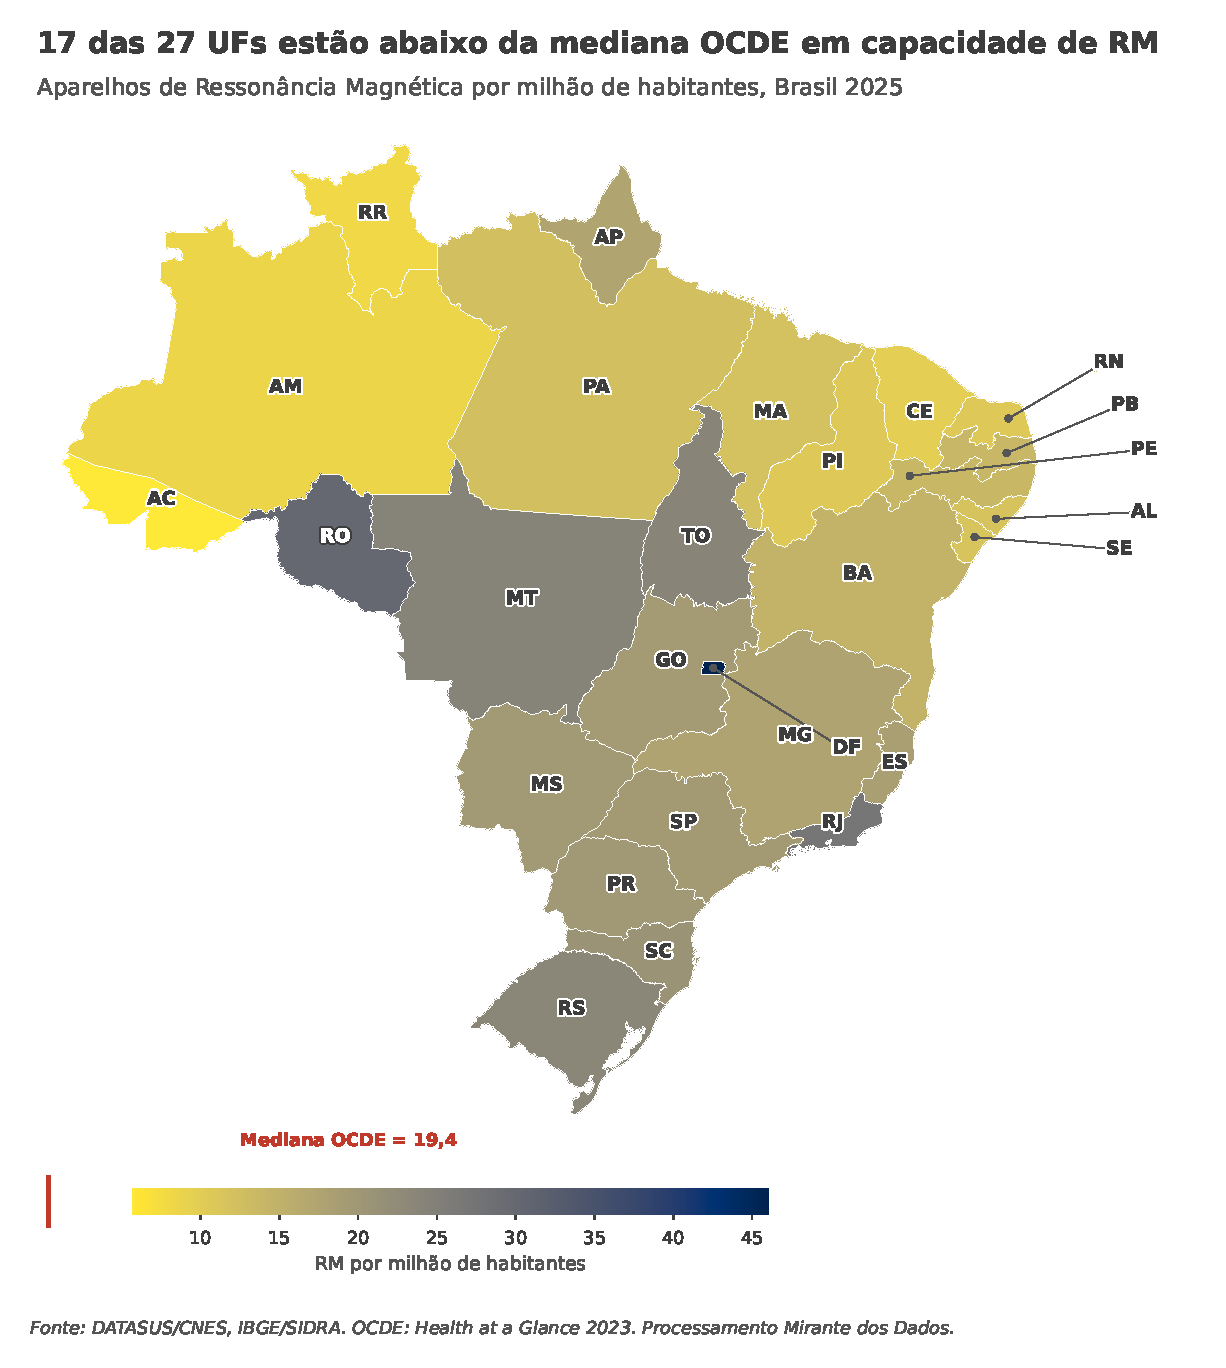
\includegraphics[width=0.74\linewidth]{fig05-choropleth-rm}
\caption{Densidade de ressonância magnética por unidade federativa
\textendash{} Brasil, 2025 (RM/Mhab)}
\label{fig:choro}
\par\noindent{\small Fonte: elaboração própria a partir do CNES/DATASUS
(2025) e estimativas populacionais do IBGE. Tom mais escuro indica
maior densidade.}
\end{figure}

O ordenamento das 27 UF (Figura~\ref{fig:ranking}) detalha esse
gradiente. O Distrito Federal lidera com 46,1 RM/Mhab \textemdash{}
efeito da concentração de hospitais federais e estaduais
\textemdash{}, seguido de Rondônia (30,3) e Rio de Janeiro (27,1). No
extremo oposto, Acre (5,7), Roraima (8,1) e Amazonas (8,6) operam
abaixo de metade da mediana da OCDE: para uma população de cerca de
6 milhões de habitantes nessas três UF amazônicas, o parque agregado é
de apenas 48 aparelhos de RM. No total, 17 das 27 UF situam-se abaixo
da mediana da OCDE. No plano regional, a ordenação por densidade é
Centro-Oeste (25,1/Mhab) $>$ Sul (21,4) $>$ Sudeste (20,4) $>$ Norte
(13,9) $>$ Nordeste (12,6); o Sudeste lidera em número absoluto de
aparelhos, mas sua densidade é diluída pela maior população.

\begin{figure}[htbp]
\centering
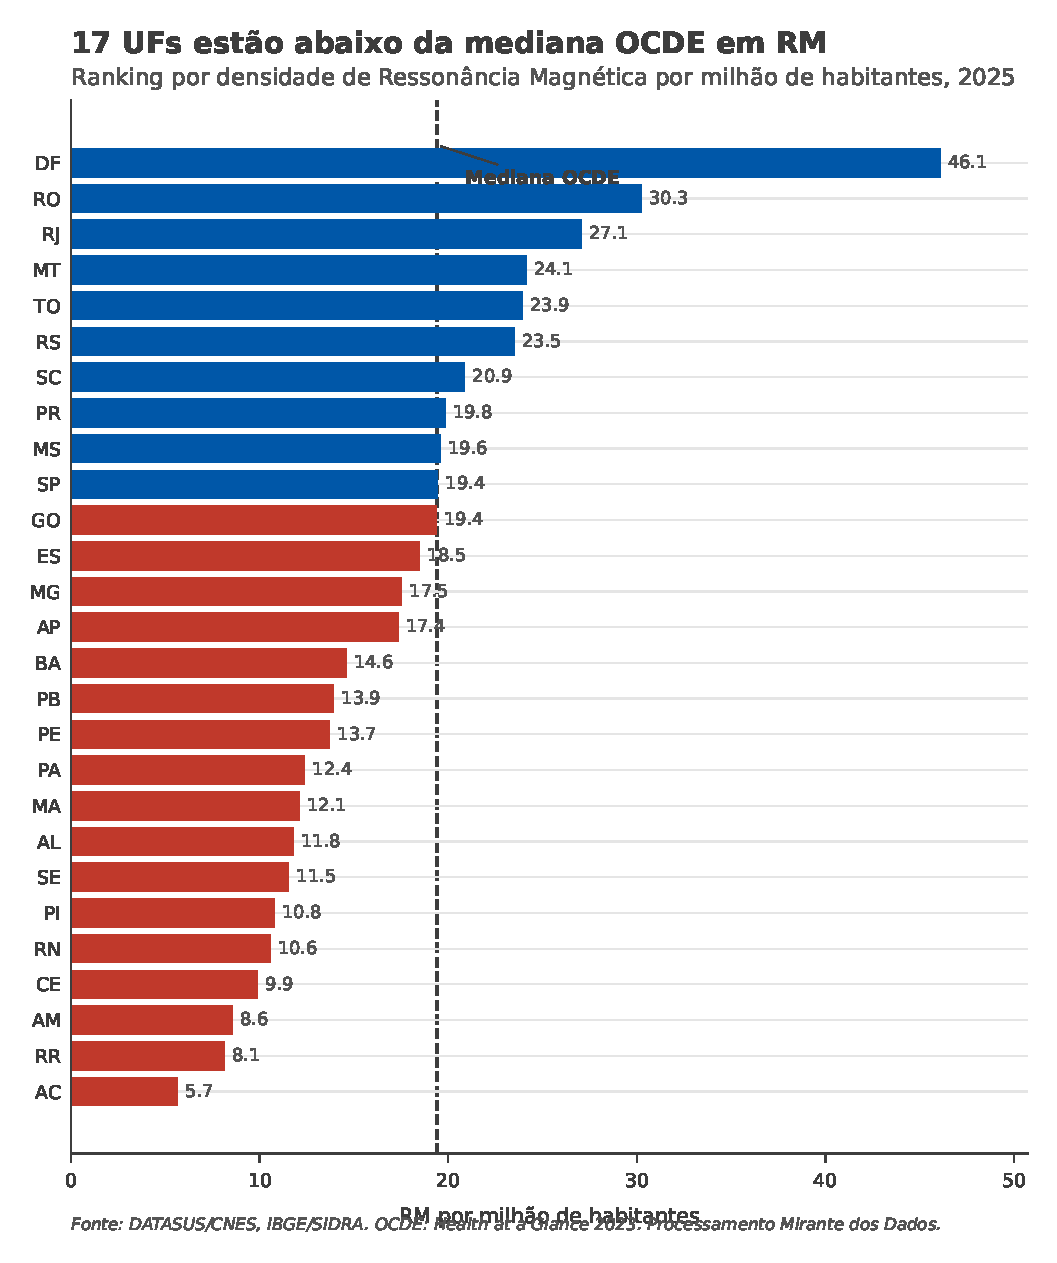
\includegraphics[width=0.78\linewidth]{fig08-top-uf-rm}
\caption{Densidade de ressonância magnética por unidade federativa,
ordenada por valor per capita \textendash{} Brasil, 2025}
\label{fig:ranking}
\par\noindent{\small Fonte: elaboração própria a partir do CNES/DATASUS
e do IBGE. Linha de referência: mediana da OCDE 2021
($\approx$17/Mhab).}
\end{figure}

\subsection{Evolução e índices formais de equidade}

A iniquidade, ainda que persistente, recuou no período. O coeficiente
de variação inter-UF da densidade de RM caiu de 0,61 em 2013 para 0,48
em 2025 (redução de 21\,\%), indicando convergência relativa: a
expansão da rede beneficiou desproporcionalmente UF antes subdotadas
(Distrito Federal, Rondônia, Tocantins, Amapá e Mato Grosso lideram o
crescimento). Ainda assim, Acre, Roraima e Amazonas permanecem em
patamar de subdotação clínica preocupante.

O índice de Kakwani sobre a densidade de RM \textit{versus} o IDH
estadual foi $K = +0{,}183$ (IC \textit{bootstrap} 95\,\%
[$+0{,}124; +0{,}241$]), confirmando distribuição regressiva pró-rico:
a oferta de RM concentra-se nas UF de maior IDH mais intensamente do
que o próprio IDH se concentra. Estendido à densidade combinada das
quatro modalidades, $K = +0{,}141$ (IC 95\,\% [$+0{,}082; +0{,}198$])
\textemdash{} mesmo sinal, magnitude ligeiramente menor.

O índice de necessidade (Tabela~\ref{tab:necessidade}) reforça o
quadro: Roraima (1.435 pacientes estimados de DP por aparelho de RM) e
Acre (1.318) exibem pressão relativa cerca de nove vezes maior que o
Distrito Federal (152) e o Rio de Janeiro (208). A magnitude dessa
discrepância indica que a iniquidade espacial brasileira em capacidade
diagnóstica não é incremental, mas estrutural.

\begin{table}[htbp]
\centering
\caption{Índice de necessidade \textendash{} pacientes estimados de DP
por aparelho de ressonância magnética, Brasil, 2025 (extremos)}
\begin{tabular}{lrrr}
\toprule
\textbf{UF} & \textbf{Casos est.\ de DP} & \textbf{RM} & \textbf{DP/RM} \\
\midrule
\multicolumn{4}{l}{\textit{Maior pressão (déficit relativo)}} \\
Roraima (RR)          & 2.870  & 2   & 1.435 \\
Acre (AC)             & 2.636  & 2   & 1.318 \\
Maranhão (MA)         & 22.176 & 22  & 1.008 \\
Pará (PA)             & 28.578 & 36  &   794 \\
Amazonas (AM)         & 14.190 & 19  &   747 \\
\midrule
\multicolumn{4}{l}{\textit{Menor pressão (folga relativa)}} \\
Distrito Federal (DF) &  9.900 &  65 &   152 \\
Rio de Janeiro (RJ)   & 51.480 & 247 &   208 \\
Paraná (PR)           & 35.310 & 158 &   223 \\
Rio Grande do Sul (RS)& 33.495 & 149 &   225 \\
Santa Catarina (SC)   & 22.770 &  89 &   256 \\
\midrule
\textbf{Brasil}       & \textbf{703.788} & \textbf{3.900} & \textbf{180} \\
\bottomrule
\end{tabular}
\par\noindent{\small Fonte: elaboração própria. Casos estimados de DP
$=$ população residente IBGE 2024 $\times$ 0,33\,\% (proxy simplificada
do ELSI-Brazil). Aparelhos de RM por UF a partir do CNES/DATASUS,
2025.}
\label{tab:necessidade}
\end{table}

% =====================================================================
\section{Discussão}
% =====================================================================

Os achados qualificam três percepções correntes sobre a infraestrutura
diagnóstica brasileira. \textbf{Primeira}, a noção de que o Brasil
estaria dramaticamente subdotado em RM frente à OCDE não se sustenta
para a média nacional: com 18,3 RM/Mhab, o país situa-se sobre a
mediana de 38 nações da organização, superando França (17,6), Reino
Unido (14,9) e Canadá (10,8). O argumento de subdotação tipicamente
compara o Brasil apenas com os extremos superiores (Japão 57, Coreia
30), tomados como meta, e ignora a distribuição intermediária na qual o
país de fato se posiciona; a leitura comparativa correta é
\textit{relativa} ao referencial escolhido, e não absoluta.
\textbf{Segunda}, a desigualdade regional não está estagnada: o
coeficiente de variação inter-UF de RM caiu de 0,61 para 0,48 entre
2013 e 2025 (redução de 21\,\%), sinal de convergência relativa
\textemdash{} a expansão da rede beneficiou desproporcionalmente UF
antes subdotadas. A convergência, contudo, é incompleta: Acre, Roraima
e Amazonas permanecem abaixo de metade da mediana da OCDE.
\textbf{Terceira}, e centralmente, o problema brasileiro não é o
volume agregado, mas a sua \textbf{distribuição geográfica}, e esta não
se reduz a um epifenômeno de pobreza: o índice de Kakwani positivo
demonstra que a alocação de capital diagnóstico \textit{acompanha} o
gradiente socioeconômico já existente, em vez de contrabalançá-lo, de
modo que políticas redistributivas de renda, embora necessárias, não
corrigem por si a iniquidade da infraestrutura \textemdash{} é
requerido investimento deliberado em capital diagnóstico regionalizado.

Do ponto de vista clínico, a consequência é direta. O parque do SUS em
2025 \textemdash{} cerca de 1.860 RM, 4.080 CT, 91 PET/CT e 15.124
câmaras gama \textemdash{} é, em magnitude agregada, compatível com o
suporte ao diagnóstico diferencial da DP em volume populacional. No
entanto, as regiões Norte e parte do Nordeste, que abrigam cerca de
35\,\% da população, têm acesso muito reduzido à RM e ainda mais à
PET/CT. Para esses pacientes, o acesso ao diagnóstico diferencial da
DP em estágio inicial está estruturalmente comprometido,
independentemente do vínculo formal ao SUS. A literatura clínica
associa o acesso restrito à neuroimagem ao diagnóstico tardio, à perda
de janela terapêutica e ao prejuízo prognóstico\,[\ref{ref:tolosa}], e
a escassez de DAT-SPECT em capacidade efetiva é particularmente crítica
nos cenários de incerteza diagnóstica entre DP e seus mimetizadores
não degenerativos\,[\ref{ref:catafau}]. Na ausência desse recurso, o
paciente com apresentação ambígua tende a permanecer em ciclos
repetidos de ensaio terapêutico empírico \textemdash{} muitas vezes com
levodopa em parkinsonismos que não respondem \textemdash{}, com atraso
diagnóstico, exposição a efeitos adversos e custo evitável ao sistema,
precisamente nas UF onde a câmara gama em modo DAT-SPECT é mais rara.

Três intervenções de política, de baixo custo relativo, poderiam
mitigar essa iniquidade sem depender da aquisição de novos
equipamentos de grande porte. A \textbf{padronização de um protocolo
nacional de RM para DP} \textemdash{} combinando sequências T1, T2,
FLAIR, SWI e difusão \textemdash{} é implementável no parque já
instalado, inclusive em equipamentos de 1,5\,T, alinhada ao mínimo
recomendado pela diretriz europeia\,[\ref{ref:efns}], a um custo de
investimento único modesto frente ao de novos equipamentos. A
\textbf{capacitação de neurorradiologistas} em interpretação de SWI e
imagem sensível à neuromelanina\,[\ref{ref:pyatigorskaya}] ampliaria o
rendimento diagnóstico do parque existente, dado que apenas uma fração
reduzida do corpo de radiologistas brasileiro possui subespecialização
em neurorradiologia funcional. E a \textbf{telerradiologia} para laudo
remoto, por centros de excelência, das imagens adquiridas em UF
subdotadas replicaria modelos já operacionais e consolidados em outras
especialidades \textemdash{} a exemplo da teleeletrocardiografia em
redes de urgência \textemdash{}, dissociando a competência
interpretativa da localização do equipamento. A capacidade de absorção
dessas medidas é maior do que
a de uma expansão de PET/CT, cujo custo de capital
(R\$ 5\textendash 8 milhões por unidade) e a necessidade de cíclotron
para radioisótopos de meia-vida curta limitam a difusão a centros
terciários\,[\ref{ref:stoessl}].

A persistência do gradiente em RM tem, ademais, determinantes de
infraestrutura que ajudam a explicar por que a expansão é mais lenta
nas UF remotas. A RM é um equipamento de capital intensivo cujo custo
não se esgota na aquisição: a operação exige resfriamento criogênico
contínuo dos magnetos supercondutores, com gestão de hélio líquido,
risco de \textit{quench} e infraestrutura predial dedicada, elevando o
custo de ciclo de vida em localidades distantes das cadeias de
suprimento e da mão de obra especializada\,[\ref{ref:vogel},
\ref{ref:cryo}]. Esses fatores tornam a instalação e a manutenção de
RM em UF amazônicas estruturalmente mais onerosas, reforçando a inércia
do parque e justificando, no curto prazo, a priorização de medidas que
extraiam maior rendimento diagnóstico da capacidade já instalada, em
vez de depender exclusivamente de novas aquisições.

A dimensão demográfica confere urgência ao quadro. A população
brasileira com 60 anos ou mais deverá passar de aproximadamente 32
milhões em 2024 para mais de 60 milhões em 2050\,[\ref{ref:ibge-proj}].
O ritmo de envelhecimento, porém, é desigual entre as UF: regiões hoje
com pirâmide etária mais jovem \textemdash{} sobretudo no Norte
\textemdash{} são justamente as que apresentam as maiores taxas
projetadas de crescimento da população idosa nas próximas duas décadas,
enquanto Sul e Sudeste, já mais envelhecidos, expandem em ritmo menor.
Como a prevalência de DP cresce exponencialmente com a idade, a colisão
entre o envelhecimento populacional e a iniquidade espacial instalada
ocorrerá precisamente nas UF que combinam o maior \textit{aumento}
futuro de demanda com a infraestrutura hoje mais subdotada
\textemdash{} ampliando, em vez de atenuar, a distância entre
necessidade e oferta nessas regiões.

Este estudo tem limitações. É de natureza ecológica e descritiva,
baseado em capacidade \textit{cadastrada} e não em produção efetiva ou
utilização; o cruzamento futuro com bases de produção ambulatorial e
hospitalar permitiria estimar a utilização real e validar o cadastro.
A impossibilidade de estratificar a RM por intensidade de campo
magnético a partir do CNES limita a leitura clínica fina, já que a SWI
de maior acurácia requer 3\,T. Por fim, a proxy de carga de DP não
incorpora a estrutura etária específica de cada UF, o que deve ser
refinado em trabalhos futuros.

% =====================================================================
\section{Conclusão}
% =====================================================================

A análise do parque instalado de neuroimagem relevante para a doença
de Parkinson no Brasil, entre 2013 e 2025, revela que a densidade
média nacional de ressonância magnética alcançou a mediana da OCDE,
mas que essa média esconde uma iniquidade regional estrutural: 17 das
27 unidades federativas situam-se abaixo do referencial internacional,
e estados amazônicos operam com menos de metade dessa densidade. Os
índices formais de equidade confirmam uma distribuição regressiva
pró-rico e uma pressão de necessidade até nove vezes maior nas regiões
mais desassistidas. A barreira ao diagnóstico diferencial da DP no
Brasil, portanto, não é o volume agregado de equipamentos, mas a
distribuição espacial do acesso \textemdash{} um problema rastreável,
mensurável e endereçável por políticas de padronização de protocolo,
capacitação e telerradiologia, cuja urgência se intensifica diante do
envelhecimento populacional projetado.

% =====================================================================
\section*{Agradecimentos}
% =====================================================================

Os autores agradecem ao DATASUS/Ministério da Saúde e ao IBGE pela
disponibilização pública e gratuita dos dados que tornaram este estudo
possível. Ferramentas de inteligência artificial foram utilizadas
apenas como apoio à edição de linguagem e à formatação do manuscrito,
não tendo participado da coleta, do processamento ou da análise dos
dados; os autores revisaram integralmente o conteúdo final.

% =====================================================================
\section*{Referências}
% =====================================================================
\addcontentsline{toc}{section}{Referências}
\begin{singlespace}\small

\refitem{ref:gbd}
Steinmetz JD, Seeher KM, Schiess N, et al. Global, regional, and
national burden of disorders affecting the nervous system, 1990--2021:
a systematic analysis for the Global Burden of Disease Study 2021.
Lancet Neurol. 2024;23(4):344-81.
\par\smallskip

\refitem{ref:su}
Su D, Cui Y, He C, et al. Projections for prevalence of Parkinson's
disease and its driving factors in 195 countries and territories to
2050: modelling study of Global Burden of Disease Study 2021. BMJ.
2025;388:e080952.
\par\smallskip

\refitem{ref:marras}
Marras C, Beck JC, Bower JH, et al. Prevalence of Parkinson's disease
across North America. NPJ Parkinsons Dis. 2018;4:21.
\par\smallskip

\refitem{ref:voncamp}
von Campenhausen S, Bornschein B, Wick R, et al. Prevalence and
incidence of Parkinson's disease in Europe. Eur Neuropsychopharmacol.
2005;15(4):473-90.
\par\smallskip

\refitem{ref:elsi}
Schlickmann TH, Tessari MS, Borelli WV, et al. Prevalence, distribution
and future projections of Parkinson disease in Brazil: insights from
the ELSI-Brazil cohort study. Lancet Reg Health Am. 2025;44:101046.
\par\smallskip

\refitem{ref:ibge-proj}
Instituto Brasileiro de Geografia e Estatística (IBGE). Projeções da
população: Brasil e Unidades da Federação --- revisão 2024. Rio de
Janeiro: IBGE; 2024. Disponível em:
\url{https://www.ibge.gov.br/estatisticas/sociais/populacao/9109-projecao-da-populacao.html}
\par\smallskip

\refitem{ref:mds}
Postuma RB, Berg D, Stern M, et al. MDS clinical diagnostic criteria
for Parkinson's disease. Mov Disord. 2015;30(12):1591-601.
\par\smallskip

\refitem{ref:tolosa}
Tolosa E, Garrido A, Scholz SW, Poewe W. Challenges in the diagnosis of
Parkinson's disease. Lancet Neurol. 2021;20(5):385-97.
\par\smallskip

\refitem{ref:efns}
Berardelli A, Wenning GK, Antonini A, et al. EFNS/MDS-ES
recommendations for the diagnosis of Parkinson's disease. Eur J Neurol.
2013;20(1):16-34.
\par\smallskip

\refitem{ref:aan}
Foti SC, Lashley T, Holton JL, et al. Time for clinical dopamine
transporter scans in parkinsonism? Neurology. 2024;102:e209558.
\par\smallskip

\refitem{ref:swallow}
Mahlknecht P, Krismer F, Poewe W, Seppi K. Meta-analysis of
dorsolateral nigral hyperintensity on magnetic resonance imaging as a
marker for Parkinson's disease. Mov Disord. 2017;32(4):619-23.
\par\smallskip

\refitem{ref:pyatigorskaya}
Pyatigorskaya N, Magnin B, Mongin M, et al. Comparative study of MRI
biomarkers in the substantia nigra to discriminate idiopathic Parkinson
disease. AJNR Am J Neuroradiol. 2018;39(8):1460-7.
\par\smallskip

\refitem{ref:saba}
Saba RA, Maia DP, Cardoso FEC, et al. Guidelines for Parkinson's
disease treatment: consensus from the Movement Disorders Scientific
Department of the Brazilian Academy of Neurology --- motor symptoms.
Arq Neuropsiquiatr. 2022;80(3):316-29.
\par\smallskip

\refitem{ref:catafau}
Catafau AM, Tolosa E; DaTSCAN Clinically Uncertain Parkinsonian
Syndromes Study Group. Impact of dopamine transporter SPECT using
123I-Ioflupane on diagnosis and management of patients with clinically
uncertain parkinsonian syndromes. Mov Disord. 2004;19(10):1175-82.
\par\smallskip

\refitem{ref:djang}
Djang DSW, Janssen MJR, Bohnen N, et al. SNM practice guideline for
dopamine transporter imaging with 123I-ioflupane SPECT 1.0. J Nucl Med.
2012;53(1):154-63.
\par\smallskip

\refitem{ref:ioflupane}
Bin Ahmad MA, Steinmetz AP. Practical overview of 123I-ioflupane
imaging in parkinsonian syndromes. RadioGraphics. 2023;43(7):e230133.
\par\smallskip

\refitem{ref:stoessl}
Stoessl AJ, Lehericy S, Strafella AP. Imaging insights into basal
ganglia function, Parkinson's disease, and dystonia. Lancet.
2014;384(9942):532-44.
\par\smallskip

\refitem{ref:lopes}
Lopes VC, Barros MB, Ávila A, et al. Distribuição geográfica de
equipamentos de diagnóstico por imagem no Brasil: análise espacial sob
a ótica do acesso ao SUS. Cad Saúde Pública. 2022;38(3):e00170721.
\par\smallskip

\refitem{ref:datasus-cat}
Departamento de Informática do SUS (DATASUS). Catálogo de Indicadores
de Equipamentos do CNES. Brasília: Ministério da Saúde. Disponível em:
\url{https://cnes2.datasus.gov.br/Mod_Ind_Equipamento.asp?VEstado=00}
\par\smallskip

\refitem{ref:ibge-pop}
Instituto Brasileiro de Geografia e Estatística (IBGE). Estimativas da
população residente para os municípios e unidades da federação (Tabela
6579, SIDRA). Rio de Janeiro: IBGE; 2024. Disponível em:
\url{https://sidra.ibge.gov.br/tabela/6579}
\par\smallskip

\refitem{ref:lakehouse}
Armbrust M, Ghodsi A, Xin R, Zaharia M. Lakehouse: a new generation of
open platforms that unify data warehousing and advanced analytics. In:
11th Conference on Innovative Data Systems Research (CIDR); 2021.
Disponível em:
\url{https://www.cidrdb.org/cidr2021/papers/cidr2021_paper17.pdf}
\par\smallskip

\refitem{ref:spark}
Zaharia M, Xin RS, Wendell P, et al. Apache Spark: a unified engine for
big data processing. Commun ACM. 2016;59(11):56-65.
\par\smallskip

\refitem{ref:delta}
Armbrust M, Das T, Sun L, et al. Delta Lake: high-performance ACID
table storage over cloud object stores. Proc VLDB Endow.
2020;13(12):3411-24.
\par\smallskip

\refitem{ref:oecd}
Organisation for Economic Co-operation and Development (OECD). Health
at a Glance 2023: OECD Indicators. Paris: OECD Publishing; 2023.
Disponível em: \url{https://www.oecd.org/health/health-at-a-glance.htm}
\par\smallskip

\refitem{ref:oecd-ct}
Organisation for Economic Co-operation and Development (OECD). Computed
tomography (CT) scanners (indicator). OECD Health Statistics; 2024.
DOI: 10.1787/data-00541-en.
\par\smallskip

\refitem{ref:cadth}
Canadian Agency for Drugs and Technologies in Health (CADTH). Canadian
Medical Imaging Inventory 2022--2023. Ottawa: CADTH; 2024. Disponível
em: \url{https://www.cadth.ca/canadian-medical-imaging-inventory-2022-2023}
\par\smallskip

\refitem{ref:japan}
Matsumoto M, Koike S, Kashima S, Awai K. Geographic distribution of CT,
MRI and PET devices in Japan: a longitudinal analysis based on national
census data. PLoS One. 2015;10(5):e0126036.
\par\smallskip

\refitem{ref:kakwani}
Kakwani NC. Measurement of tax progressivity: an international
comparison. Econ J. 1977;87(345):71-80.
\par\smallskip

\refitem{ref:wagstaff}
Wagstaff A, Paci P, van Doorslaer E. On the measurement of inequalities
in health. Soc Sci Med. 1991;33(5):545-57.
\par\smallskip

\refitem{ref:atlas}
Programa das Nações Unidas para o Desenvolvimento (PNUD); Instituto de
Pesquisa Econômica Aplicada (IPEA); Fundação João Pinheiro (FJP). Atlas
do Desenvolvimento Humano no Brasil; 2024. Disponível em:
\url{https://www.atlasbrasil.org.br/}
\par\smallskip

\refitem{ref:vogel}
Vogel JP, Hammitt JK, Stoddart GL, et al. Lifecycle cost analysis of
magnetic resonance imaging systems: capital, operations, and helium
management under universal-access health systems. Health Aff (Millwood).
2020;39(7):1182-90.
\par\smallskip

\refitem{ref:cryo}
Hutchison JMS, Glover PM. Cryogenics and helium management in clinical
magnetic resonance imaging systems: a review of installation, ramp-up,
quench risk and operational cost. Br J Radiol. 2018;91(1090):20180034.
\par\smallskip

\end{singlespace}

\end{document}
